
%%
%% Historical context
%%

\begin{frame}[fragile]{The quadratic equation}

\begin{columns}

  \begin{column}{7.5cm}
  \begin{itemize}
  \item Methods for finding the positive roots of the
    positive-coefficients quadratic equation appear in Babylonian clay
    tablets from 21st~c. BC.
  \item In the 9th c. al-Khwarizmi proves formulas that calculate the
    positive solution(s) as functions of positive, rational coefficients
  \item In the 13th c. Yang Hui solves quadratic equations with
    negative coefficients
  \item Ren{\' e} Descartes' \emph{La G{\' e}om{\' e}trie} (1637)
    gives the quadratic formula in the form we know today
  \end{itemize}
  \end{column}

  \begin{column}{4.5cm}
  \includegraphics[width=4cm]{contents/images/descartes}
  \end{column}

\end{columns}

\end{frame}

  

\begin{frame}{The cubic and quartic equations}

\begin{columns}

  \begin{column}{7.5cm}
  \begin{itemize}
  \item Ancient solutions or almost-solutions for specific cases:
    doubling the cube, Diophantine equations, conic sections
  \item 11th c. Omar Khayyam: geometric solution, realizes multiple
    solution exist, tries and fails algebraic formulation of the
    solution
  \item Scipione del Ferro solves $x^3 + mx = n$, not
    realizing it is general
  \item Girolamo Cardano realizes (1545) del Ferro's solution and
    Lodovico Ferrari's quartic solution are general
  \item Descartes gives the modern formulas (1637)
  \end{itemize}
  \end{column}

  \begin{column}{4.5cm}
    \begin{tikzpicture}
      \node (descartes) {\includegraphics[width=3cm]{contents/images/descartes}};
      \node (cardano) at (descartes.south west)
            {\includegraphics[width=4cm]{contents/images/cardano}};
    \end{tikzpicture}
  \end{column}

\end{columns}

\end{frame}



\begin{frame}{The end of the path}

\begin{columns}

  \begin{column}{7.5cm}
  \begin{itemize}
  \item Paolo Ruffini (1799, 1813) and Niels Henrik Abel (1824) prove
    that there is no algebraic solution to indeterminate equations of
    degree five or higher \vspace{0.5em}
  \item Galois Theory (1830, 1846) implies that there are equations of
    degree five and higher that do not have algebraic solution \vspace{0.2em}
    \begin{itemize}
    \item Almost all polynomials cannot be solved \vspace{0.1em}
    \item $x^{5}-x-1=0$ simplest unsolvable polynomial
    \end{itemize}
  \end{itemize}
  \end{column}

  \begin{column}{4.5cm}
    \begin{tikzpicture}
      \node (descartes) {\includegraphics[width=2cm]{contents/images/descartes}};
      \node (cardano) at ([xshift=0.3cm] descartes.south west)
            {\includegraphics[width=3cm]{contents/images/cardano}};
      \node (galois) at ([xshift=0.5cm,yshift=0.5cm] cardano.south west)
            {\includegraphics[width=4cm]{contents/images/galois}};
    \end{tikzpicture}
  \end{column}

\end{columns}

\end{frame}



\begin{frame}{Hilbert's 13th}

\begin{columns}

  \begin{column}{7.5cm}
  \begin{itemize}
  \item Since Tschirnhaus (1683) it is known that every 7th-degree can be
    algebraically reduced to $x^{7}+ax^{3}+bx^{2}+cx+1=0$
  \item Algebraic solutions are functions of three variables
  \item \emph{Can this be expressed as the composition of a finite number
    of two-variable functions?} (Hilbert 1900, 1902)
  \item Following up on a series of post-Galois results on trying to
    understand high-order algebraic polynomial equations
  \end{itemize}
  \end{column}

  \begin{column}{4.5cm}
    \begin{tikzpicture}
      \node (cardano) {\includegraphics[width=2cm]{contents/images/cardano}};
      \node (galois) at ([xshift=0.3cm] cardano.south west)
            {\includegraphics[width=3cm]{contents/images/galois}};
      \node (hilbert) at ([xshift=0.5cm,yshift=0.5cm] galois.south west)
            {\includegraphics[width=4cm]{contents/images/hilbert}};
    \end{tikzpicture}
  \end{column}

\end{columns}

\end{frame}



\begin{frame}{Kolmogorov and Arnold's results}

\begin{columns}

  \begin{column}{7cm}
  \begin{itemize}
  \item Kolmogorov (1956): Every continuous multi-variable function
    can be expressed as the composition of a finite number of
    three-variable functions \vspace{0.3em}
  \item Arnold (1957): Only two-variable functions are really needed \vspace{0.3em}
  \item Kolmogorov (1957): Actually, the only two-variable function
    needed is addition \vspace{0.3em}
  \item This is a generalization of Hilbert's question, but the
    univariate functions are not necessarily algebraic
  \end{itemize}
  \end{column}

  \begin{column}{5cm}
    \begin{tikzpicture}
      \node (galois) {\includegraphics[width=2cm]{contents/images/galois}};
      \node (hilbert) at ([xshift=0.3cm] galois.south east)
            {\includegraphics[width=3cm]{contents/images/hilbert}};
      \node (kolmogorov) at ([xshift=-1cm,yshift=0.5cm] hilbert.south west)
            {\includegraphics[width=3cm]{contents/images/kolmogorov}};
      \node (arnold) at ([xshift=-0.3cm,yshift=0.5cm] hilbert.south east)
            {\includegraphics[width=3cm]{contents/images/arnold}};
    \end{tikzpicture}
  \end{column}

\end{columns}

\end{frame}



\begin{frame}{Kolmogorov-Arnold Representation Theorem}

\begin{columns}

  \begin{column}{6cm}
  \begin{itemize}
  \item Every multi-variate continuous function $f$ can be
    written using only univariate functions and addition:
    $$
    f(x_{i=1..n}) = \sum_{q=0}^{2n}\phi_q\left(\sum_{p=1}^n\psi_{q,p}(x_p)\right)
    $$
  \item In other words, addition is the only real multi-variate function,
    everything else is syntactic sugar
  \end{itemize}
  \end{column}

  \begin{column}{7cm}
  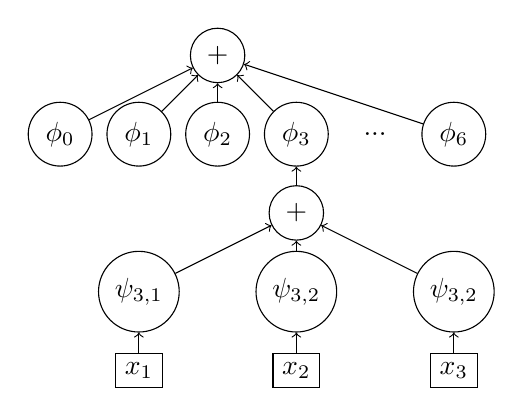
\begin{tikzpicture}
    \node[shape=circle,draw=black] (sum) at (0,0) {+};

    \node[shape=circle,draw=black] (F0) at (-2,-1) {$\phi_0$};
    \path [->] (F0) edge (sum);
    \node[shape=circle,draw=black] (F1) at (-1,-1) {$\phi_1$};
    \path [->] (F1) edge (sum);
    \node[shape=circle,draw=black] (F2) at (0,-1) {$\phi_2$};
    \path [->] (F2) edge (sum);
    \node[shape=circle,draw=black] (F3) at (1,-1) {$\phi_3$};
    \path [->] (F3) edge (sum);
    \node[shape=rectangle,draw=white] (dots) at (2,-1) {$...$};
    \node[shape=circle,draw=black] (F6) at (3,-1) {$\phi_6$};
    \path [->] (F6) edge (sum);

    \node[shape=circle,draw=black] (sum2) at (1,-2) {+};
    \path [->] (sum2) edge (F3);

    \node[shape=circle,draw=black] (f31) at (-1,-3) {$\psi_{3,1}$};
    \path [->] (f31) edge (sum2);
    \node[shape=circle,draw=black] (f32) at (1,-3) {$\psi_{3,2}$};
    \path [->] (f32) edge (sum2);
    \node[shape=circle,draw=black] (f33) at (3,-3) {$\psi_{3,2}$};
    \path [->] (f33) edge (sum2);

    \node[shape=rectangle,draw=black] (x1) at (-1,-4) {$x_1$};
    \path [->] (x1) edge (f31);
    \node[shape=rectangle,draw=black] (x2) at (1,-4) {$x_2$};
    \path [->] (x2) edge (f32);
    \node[shape=rectangle,draw=black] (x3) at (3,-4) {$x_3$};
    \path [->] (x3) edge (f33);

  \end{tikzpicture}
  \end{column}

\end{columns}

\end{frame}



\begin{frame}{Sprecher Formulation}

\begin{columns}

  \begin{column}{6cm}
  Sprecher (1972) gives an alternative formulation with a single function
  at the lower layer:
  $$
  f(x_{i=1..n}) = \sum_{q=0}^{2n}\phi_q\left(\sum_{p=1}^n\lambda^{p-1}\psi(x_p+q\cdot\epsilon)+q\right)
  $$
  where $\phi_q$ are continuous,
  $\psi$ is monotonically increasing and Lipschitz-1 continuous,
  $\lambda$ and $\psi$ depend only on $n$ and not on $f$,
  and $\epsilon$ is any non-zero constant
  \end{column}

  \begin{column}{7cm}
  \begin{tikzpicture}
  \node[shape=circle,draw=black] (sum) at (0,0) {+};

  \node[shape=circle,draw=black] (F0) at (-2,-1) {$\phi_0$};
  \path [->] (F0) edge (sum);
  \node[shape=circle,draw=black] (F1) at (-1,-1) {$\phi_1$};
  \path [->] (F1) edge (sum);
  \node[shape=circle,draw=black] (F2) at (0,-1) {$\phi_2$};
  \path [->] (F2) edge (sum);
  \node[shape=circle,draw=black] (F3) at (1,-1) {$\phi_3$};
  \path [->] (F3) edge (sum);
  \node[shape=rectangle,draw=white] (dots) at (2,-1) {$\dots$};
  \node[shape=circle,draw=black] (F6) at (3,-1) {$\phi_6$};
  \path [->] (F6) edge (sum);

  \node[shape=circle,draw=black] (sum2) at (-1,-2) {+};
  \path [->] (sum2) edge (F1);

  \node[shape=rectangle,draw=black,fill=white] (l1) at (-1.8,-3) {$\psi(x_1+\epsilon)+1$};
  \node[shape=rectangle,draw=black,fill=white] (l2) at (-1.2,-3.8) {$\lambda\psi(x_2+\epsilon)+1$};
  \node[shape=rectangle,draw=black,fill=white] (l3) at (0,-4.6) {$\lambda^2\psi(x_3+\epsilon)+1$};
  \begin{scope}[on background layer]
    \path [->, behind path] (l1) edge (sum2);
    \path [->, behind path] (l2) edge (sum2);
    \path [->] (l3) edge (sum2);
  \end{scope}
    
  \node[shape=circle,draw=black] (sum4) at (1,-2) {+};
  \path [->] (sum4) edge (F3);

  \node[shape=rectangle,draw=black,fill=white] (l1) at (1,-3) {$\psi(x_1+3\epsilon)+3$};
  \node[shape=rectangle,draw=black,fill=white] (l2) at (1.8,-3.8) {$\lambda\psi(x_2+3\epsilon)+3$};
  \node[shape=rectangle,draw=black,fill=white] (l3) at (3.2,-4.6) {$\lambda^2\psi(x_3+3\epsilon)+3$};
  \begin{scope}[on background layer]
    \path [->] (l1) edge (sum4);
    \path [->] (l2) edge (sum4);
    \path [->] (l3) edge (sum4);
  \end{scope}

\end{tikzpicture}

  \end{column}

\end{columns}

\end{frame}



\begin{frame}{Some Thoughts and Intuitions}

\begin{itemize}
\item The theorem premises that $x_i$ are in the unit interval---this
  is needed for some of the constructions in the proof and is not a
  real restriction \vspace{0.5em}
\item The theorem proves the existence of the $\phi$ and $\psi$
  functions, does not tell you how to construct them \vspace{0.5em}
\item We know very little about $\phi$ (continuous) and slightly more
  (but still little) about $\psi$ (monotonic increasing and
  Lip-1 continuous) \vspace{0.5em}
\item It is unlikely that these functions can be defined by a
  neat-looking closed formula
\end{itemize}

\end{frame}



\begin{frame}{Some Thoughts and Intuitions}

\begin{columns}

  \begin{column}{6cm}
  \begin{itemize}
  \item Sprecher notes that he uses $\lambda^p$ but other non-linear
    sequences also work \vspace{0.5em}
  \item Feels like the $n$ values in the unit interval are
    \quotes{packed} into a single value in $\mathcal{R}$ and then
    \quotes{decoded} by the $\phi$ functions \vspace{0.3em}
    \begin{itemize}
    \item Note how $\lambda$ depends on $n$
    \end{itemize}
  \end{itemize}
  \end{column}

  \begin{column}{7cm}
  \begin{tikzpicture}
  \node[shape=circle,draw=black] (sum) at (0,0) {+};

  \node[shape=circle,draw=black] (F0) at (-2,-1) {$\phi_0$};
  \path [->] (F0) edge (sum);
  \node[shape=circle,draw=black] (F1) at (-1,-1) {$\phi_1$};
  \path [->] (F1) edge (sum);
  \node[shape=circle,draw=black] (F2) at (0,-1) {$\phi_2$};
  \path [->] (F2) edge (sum);
  \node[shape=circle,draw=black] (F3) at (1,-1) {$\phi_3$};
  \path [->] (F3) edge (sum);
  \node[shape=rectangle,draw=white] (dots) at (2,-1) {$\dots$};
  \node[shape=circle,draw=black] (F6) at (3,-1) {$\phi_6$};
  \path [->] (F6) edge (sum);

  \node[shape=circle,draw=black] (sum2) at (-1,-2) {+};
  \path [->] (sum2) edge (F1);

  \node[shape=rectangle,draw=black,fill=white] (l1) at (-1.8,-3) {$\psi(x_1+\epsilon)+1$};
  \node[shape=rectangle,draw=black,fill=white] (l2) at (-1.2,-3.8) {$\lambda\psi(x_2+\epsilon)+1$};
  \node[shape=rectangle,draw=black,fill=white] (l3) at (0,-4.6) {$\lambda^2\psi(x_3+\epsilon)+1$};
  \begin{scope}[on background layer]
    \path [->, behind path] (l1) edge (sum2);
    \path [->, behind path] (l2) edge (sum2);
    \path [->] (l3) edge (sum2);
  \end{scope}
    
  \node[shape=circle,draw=black] (sum4) at (1,-2) {+};
  \path [->] (sum4) edge (F3);

  \node[shape=rectangle,draw=black,fill=white] (l1) at (1,-3) {$\psi(x_1+3\epsilon)+3$};
  \node[shape=rectangle,draw=black,fill=white] (l2) at (1.8,-3.8) {$\lambda\psi(x_2+3\epsilon)+3$};
  \node[shape=rectangle,draw=black,fill=white] (l3) at (3.2,-4.6) {$\lambda^2\psi(x_3+3\epsilon)+3$};
  \begin{scope}[on background layer]
    \path [->] (l1) edge (sum4);
    \path [->] (l2) edge (sum4);
    \path [->] (l3) edge (sum4);
  \end{scope}

\end{tikzpicture}

  \end{column}

\end{columns}

\end{frame}



\begin{frame}{Some Thoughts and Intuitions}

\begin{columns}

  \begin{column}{6cm}
  \begin{itemize}
  \item $\psi$ has many `intervals' and translating by $q\cdot\epsilon$
    lands $x_i$ into the right interval
    \begin{itemize}
    \item hacks the multiple $\psi_i$ functions into one that
      behaves differently in each interval
    \end{itemize}
  \item The lower level `packs' the effect of~$f$ on~$x_i$ for
    different values of the other inputs $x_{j\neq i}$
  \item The upper level decodes to deliver the output
  \end{itemize}
  \end{column}

  \begin{column}{7cm}
  \begin{tikzpicture}
  \node[shape=circle,draw=black] (sum) at (0,0) {+};

  \node[shape=circle,draw=black] (F0) at (-2,-1) {$\phi_0$};
  \path [->] (F0) edge (sum);
  \node[shape=circle,draw=black] (F1) at (-1,-1) {$\phi_1$};
  \path [->] (F1) edge (sum);
  \node[shape=circle,draw=black] (F2) at (0,-1) {$\phi_2$};
  \path [->] (F2) edge (sum);
  \node[shape=circle,draw=black] (F3) at (1,-1) {$\phi_3$};
  \path [->] (F3) edge (sum);
  \node[shape=rectangle,draw=white] (dots) at (2,-1) {$\dots$};
  \node[shape=circle,draw=black] (F6) at (3,-1) {$\phi_6$};
  \path [->] (F6) edge (sum);

  \node[shape=circle,draw=black] (sum2) at (-1,-2) {+};
  \path [->] (sum2) edge (F1);

  \node[shape=rectangle,draw=black,fill=white] (l1) at (-1.8,-3) {$\psi(x_1+\epsilon)+1$};
  \node[shape=rectangle,draw=black,fill=white] (l2) at (-1.2,-3.8) {$\lambda\psi(x_2+\epsilon)+1$};
  \node[shape=rectangle,draw=black,fill=white] (l3) at (0,-4.6) {$\lambda^2\psi(x_3+\epsilon)+1$};
  \begin{scope}[on background layer]
    \path [->, behind path] (l1) edge (sum2);
    \path [->, behind path] (l2) edge (sum2);
    \path [->] (l3) edge (sum2);
  \end{scope}
    
  \node[shape=circle,draw=black] (sum4) at (1,-2) {+};
  \path [->] (sum4) edge (F3);

  \node[shape=rectangle,draw=black,fill=white] (l1) at (1,-3) {$\psi(x_1+3\epsilon)+3$};
  \node[shape=rectangle,draw=black,fill=white] (l2) at (1.8,-3.8) {$\lambda\psi(x_2+3\epsilon)+3$};
  \node[shape=rectangle,draw=black,fill=white] (l3) at (3.2,-4.6) {$\lambda^2\psi(x_3+3\epsilon)+3$};
  \begin{scope}[on background layer]
    \path [->] (l1) edge (sum4);
    \path [->] (l2) edge (sum4);
    \path [->] (l3) edge (sum4);
  \end{scope}

\end{tikzpicture}

  \end{column}

\end{columns}

\end{frame}
